\section{CLUE in the CMSSW}
\label{sec:cmsswClue}


The future High Luminosity LHC (HL-LHC) is expected to deliver about 5 times higher instantaneous luminosity than the present LHC, resulting in pile-up up to 200 interactions per bunch crossing (PU200). As part of the phase-II upgrade program, the CMS collaboration is developing a new end-cap calorimeter system, the High Granularity Calorimeter (HGCAL), featuring highly-segmented hexagonal silicon sensors and scintillators with more than 6 million channels. For each event, the HGCAL clustering algorithm needs to group more than $10^5$ hits into clusters. As consequence of both high pile-up and the high granularity, the HGCAL clustering algorithm is confronted with an unprecedented computing load. CLUE (CLUsters of Energy) is a fast fully-parallelizable density-based clustering algorithm, optimized for high pile-up scenarios in high granularity calorimeters. In this paper, we present both CPU and GPU implementations of CLUE in the application of HGCAL clustering in the CMS Software framework (CMSSW). Comparing with the previous HGCAL clustering algorithm, CLUE on CPU (GPU) in CMSSW is 30x (180x) faster in processing PU200 events while outputting almost the same clustering results.


\subsection{Implementation in the CMSSW}



% image algo
The previous clustering algorithm \cite{Chen:2017btc} used in the CMS HGCAL reconstruction was based on Clustering by Fast Search and Find Density Peak (CFSFDP) \cite{rodriguez2014clustering} and exploited a KD-Tree spatial index \cite{Bentley:1975:MBS:361002.361007}. In the step of calculating local density $\rho$, KD-Tree provides a significant speedup comparing with not using any spatial index \cite{Chen:2017btc}. However, it has three crucial computing weaknesses: first, KD-Tree does not provide the optimal spatial index for HGCAL, because its window-query is of $O(n\log n)$ complexity and it is hard to construct or query on the GPUs; second, the calculation of separation $\delta$ does not take advantage of spatial index but still relies on a costly $O(n^2)$ loop; third, the expansion of clusters happens in sequential order of decreasing density, which is not only costly because of sorting but also hard to parallelize.


% clue
CLUsters of Energy (CLUE) \cite{cluepaper} is a recently-proposed parallelizable high-speed clustering algorithm. It overcomes the above three computing weaknesses and achieves an average $O(n)$ computational complexity in the applications like HGCAL where $n> k \gg m$. CLUE uses a spatial index \cite{bentley1979data} for fast querying of neighbours. Figure \ref{fig:algorithm:procedure} is a demonstration of CLUE procedure provided in \cite{cluepaper}. Both the CPU and the GPU version of CLUE, referred as CLUE-CPU and CLUE-GPU in this paper, have been implemented in CMSSW for HGCAL reconstruction. CLUE-CPU is implemented in C++, while CLUE-GPU is implemented using CUDA. Figure~\ref{fig:cmssw} shows the workflow of CLUE-GPU within CMSSW: hits are offloaded from CPU to GPU after energy calibration; then CLUE steps are carried out on GPU; in the end, the clustering results are transported back to CPU for post processing and other downstream HGCAL reconstruction related to 3D linkage of CLUE clusters. 

% \begin{figure}[ht]
%     \centering
%     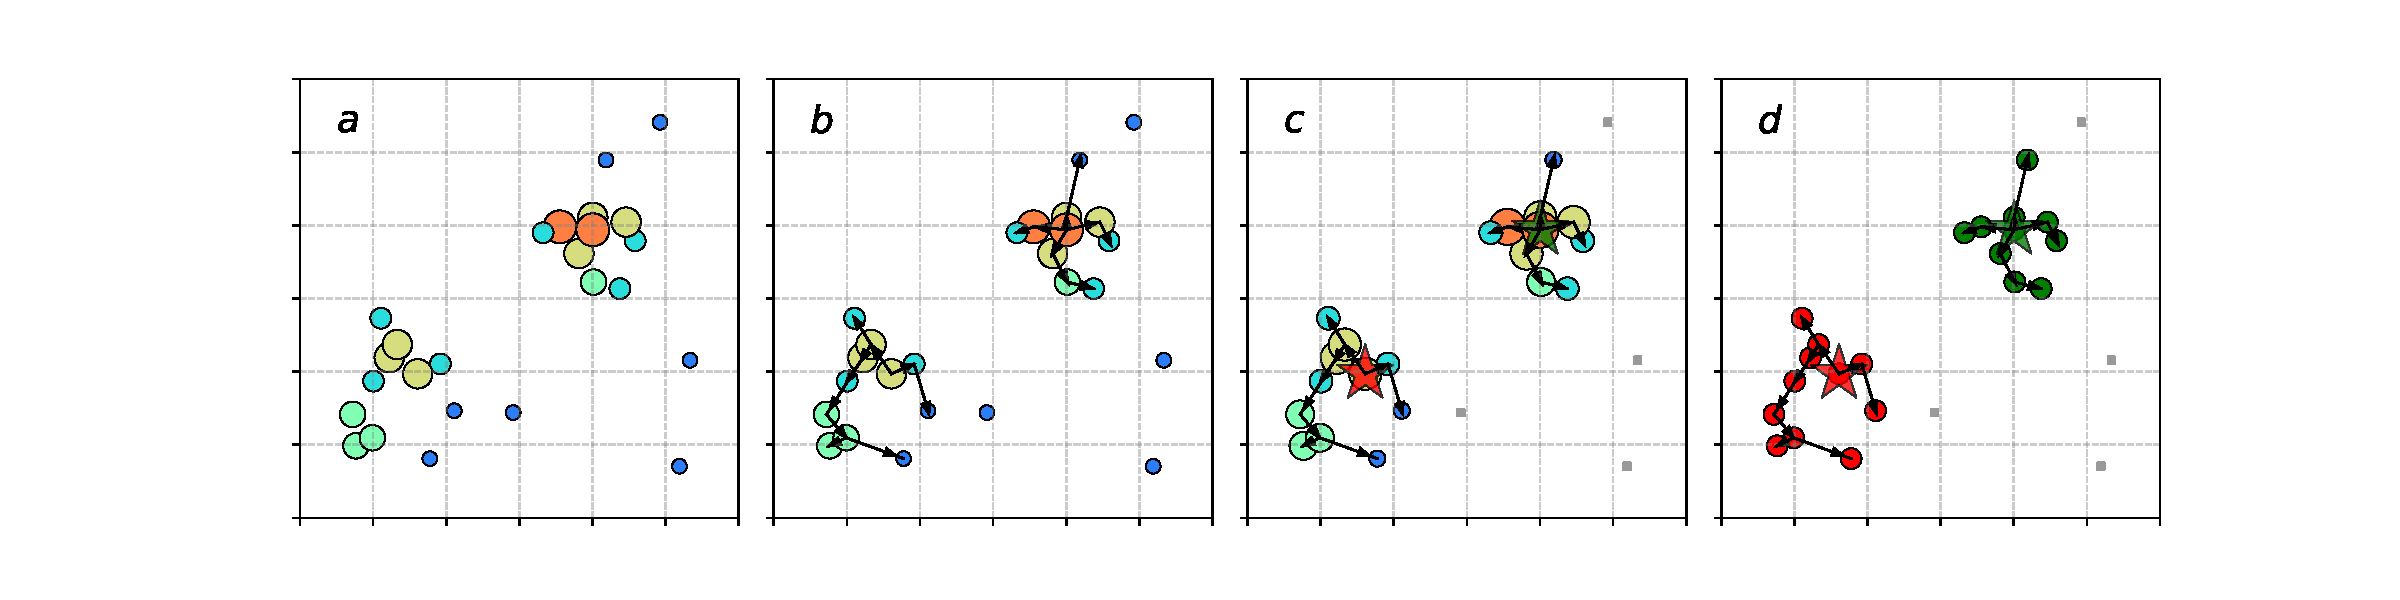
\includegraphics[trim=5cm 0cm 4cm 0cm, clip,width=0.99\textwidth]{chapters/HGCal/figures/chep/Figure2.pdf}
%     \caption{Demonstration of CLUE procedure \cite{cluepaper}. The definitions of four internal variables $\{ \rho, \delta, nh, followers\}$ are also given in \cite{cluepaper}. Before the clustering procedure starts, a fixed-grid spatial index is constructed. In the first step, shown as (a), CLUE calculates the local density $\rho$ for each point. The color and size of points represent their local densities. In the second step, shown as (b), for each point CLUE calculates its nearest-higher $nh$ (defined as the nearest hit with higher density) and its separation $\delta$ (defined as the distance to $nh$). The black arrows represent the relation from the nearest-higher of a point to the point itself. If the nearest-higher of a point is -1, there is no arrow pointing to it. In the third step, shown as (c), CLUE promotes a point as a seed if $\rho,\delta$ are both large, or demote it to an outlier if $\rho$ is small and $\delta$ is large. Promoted seeds and demoted outliers are shown as stars and grey squares, respectively. In the fourth step, shown as (d), CLUE propagates the cluster indices from seeds through their chains of followers. Noise points, which are outliers and their descendant followers, are guaranteed not to receive cluster ids from any seeds. The color of points represents the cluster ids. A grey square means its cluster id is undefined and the point should be considered as noise.
%     }
%     \label{fig:algorithm:procedure}
% \end{figure}


\begin{figure}[ht]
    \centering
    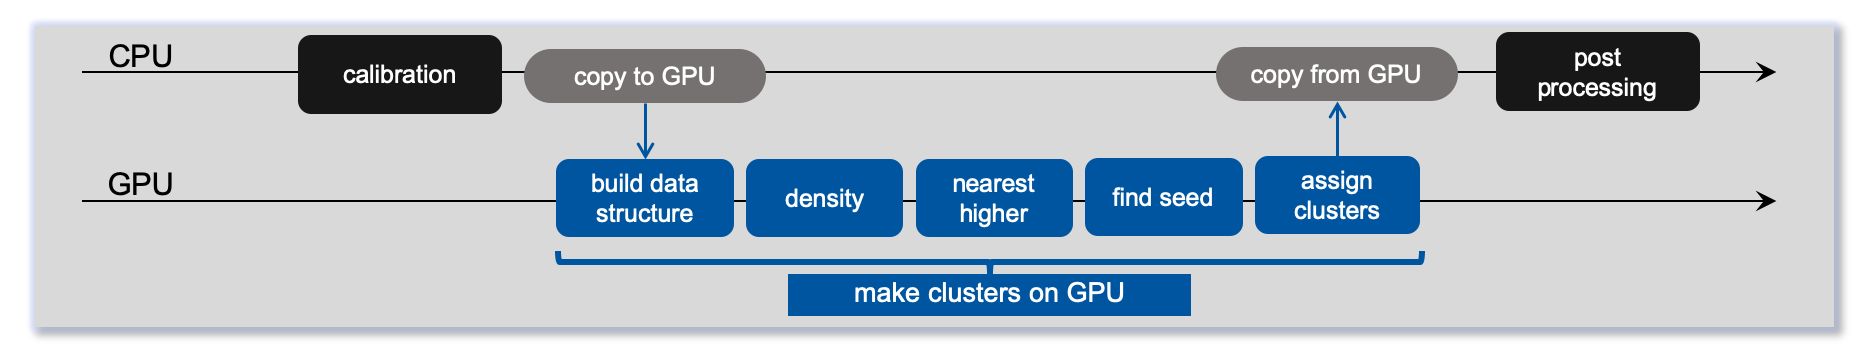
\includegraphics[trim=0.5cm 0cm 0.5cm 0cm, clip,width=0.99\textwidth]{chapters/HGCal/figures/chep/CMSSWFollow.png}
    \caption{ Workflow of CLUE-GPU in CMSSW. Hits are offloaded from CPU to GPU after energy calibration. Then CLUE process are carried out on GPU. In the end, the cluster indices of all hits are transported back to CPU for post processing.}
    \label{fig:cmssw}
\end{figure}


% validate CLUE result
\begin{figure}[ht]
    \centering
    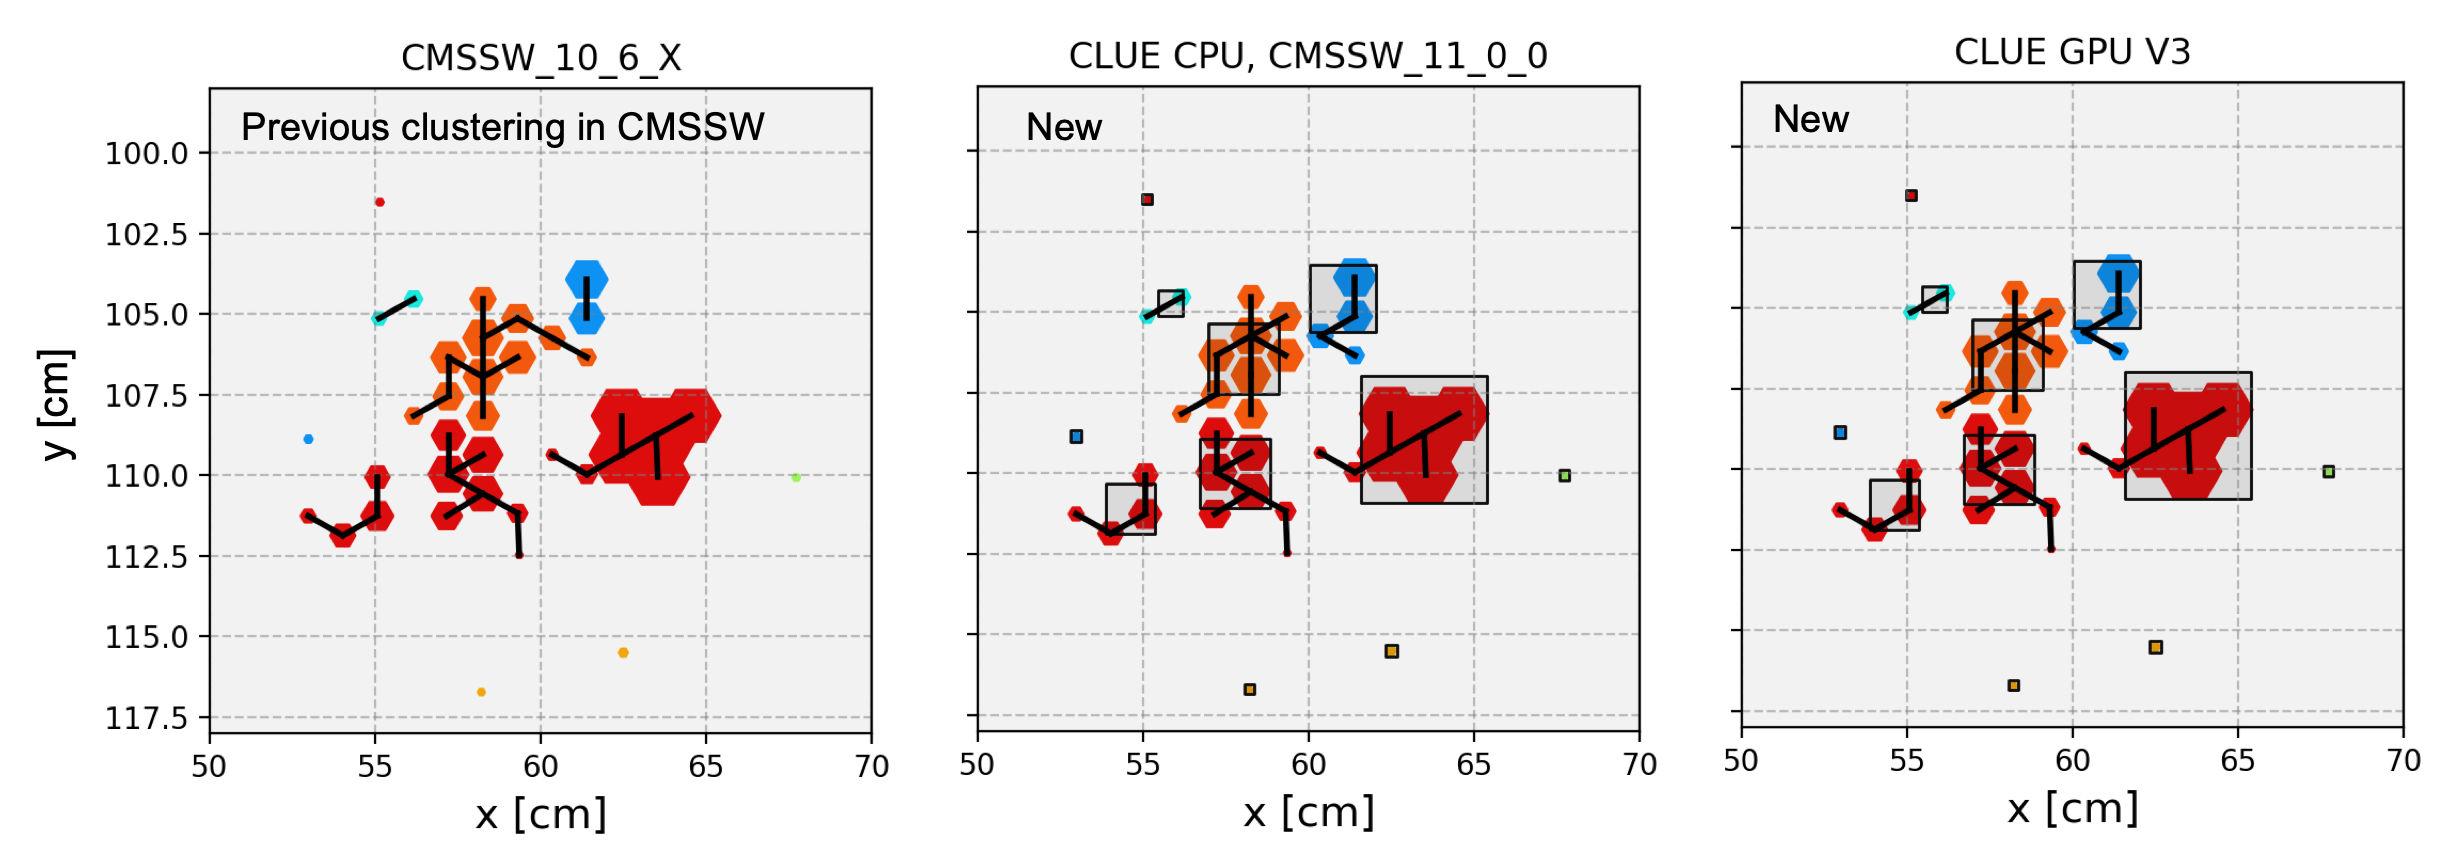
\includegraphics[trim=0cm 0cm 0cm 0cm, clip, width=0.90\textwidth]{chapters/HGCal/figures/chep/results.png}
    \caption{ Example of clustering result from previous algorithm in CMSSW\_10\_6\_X (\emph{left}) and CLUE-CPU (\emph{middle}) and CLUE-GPU (\emph{right}). The example shows a small region on the 12$^{th}$ layer of a simulated of $t\bar{t}$ event.
    }
    \label{fig:results}
\end{figure}

To validate the implementation of CLUE in CMSSW, results of CLUE-CPU and CLUE-GPU are compared with the previous clustering algorithm in CMSSW version 10.6, referred as CMSSW\_10\_6\_X. Based on the simulated $t\bar{t}$ events, CLUE-CPU and CLUE-GPU completely agree with each other, while both of them show some rare disagreements with the previous clustering algorithm implemented in CMSSW\_10\_6\_X. Such disagreements are caused by the different ordering of hits with exactly equal $\rho$ or equal $\delta$ when using different data structures, namely grid in CLUE and KD-Tree in CMSSW\_10\_6\_X. An example of clustering result is shown in Figure~\ref{fig:results}, where from left to right are results from CMSSW\_10\_6\_X, CLUE-CPU and CLUE-GPU. In this example, CLUE-CPU and CLUE-GPU provide almost the same result as the clusters in CMSSW\_10\_6\_X. However, a small notable difference is the blue cluster, which includes 4 hits in CMSSW\_10\_6\_X but 2 in CLUE. This is because the hit at about (x=60, y=106) cm is equally close to the two neighbouring hits in orange cluster and blue cluster, and its two different assignments, caused by different ordering of these two neighbors in spatial index, are equally correct. The topology of blue cluster in both cases are acceptable. Therefore, it is reasonable to conclude that CLUE in CMSSW gives almost the same clustering result as CMSSW\_10\_6\_X with neglectable differences.





\subsection{Performance in the CMSSW}


\begin{figure}[ht]
    \centering
    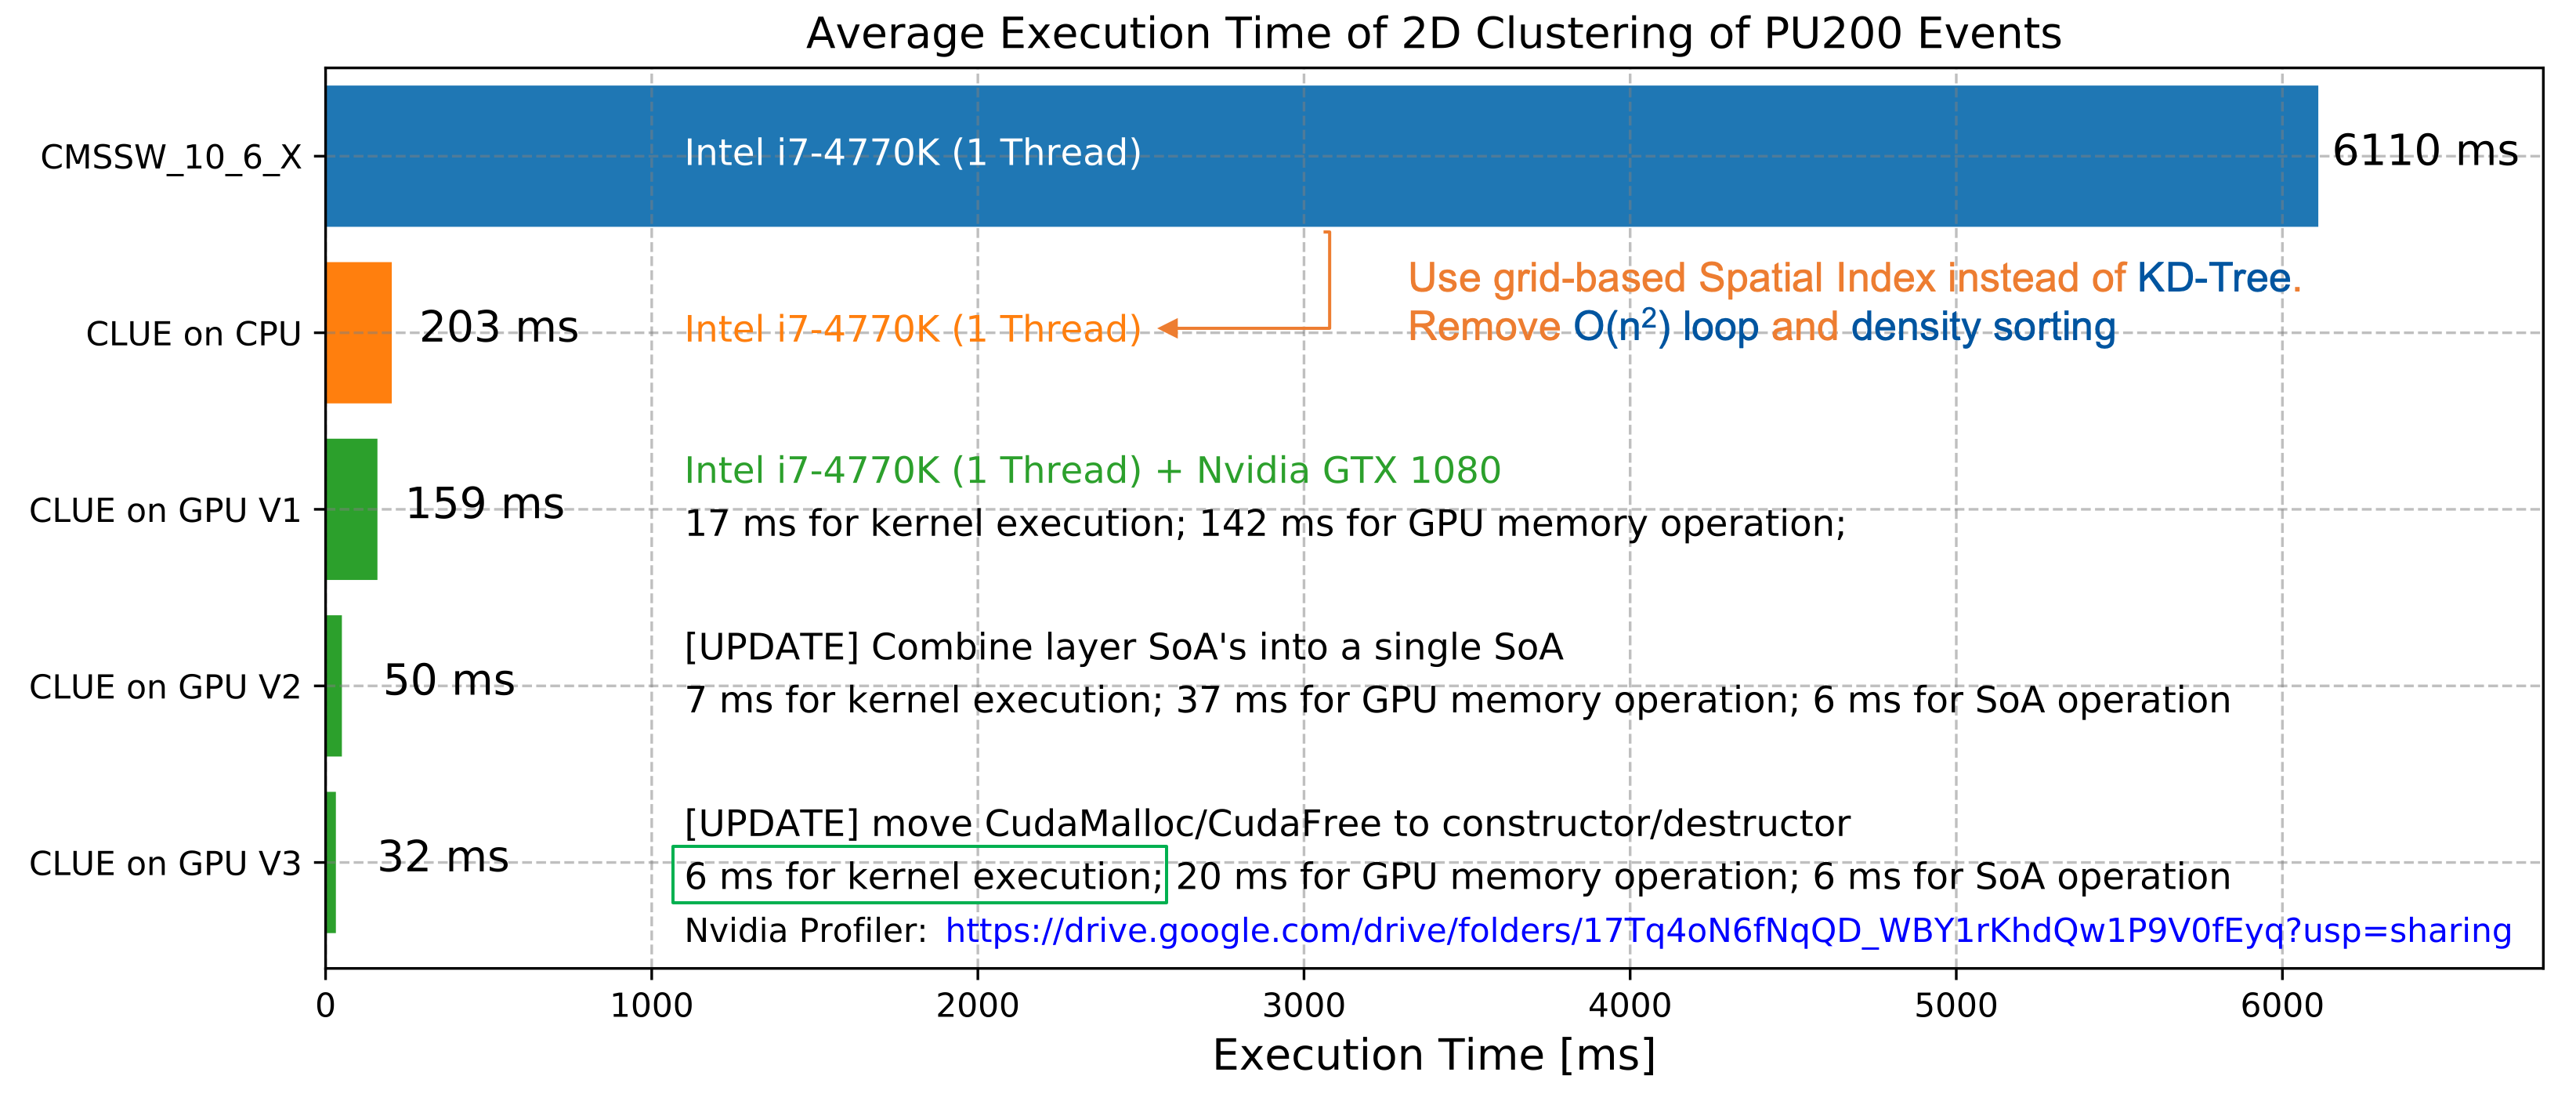
\includegraphics[trim=0cm 0cm 0cm 0cm, clip,width=0.99\textwidth]{chapters/HGCal/figures/chep/performance.png}
    \caption{ 
    Average execution time of HGCAL clustering for PU200 events. The testing platform is based on Intel i7-4770K CPU and NVIDIA GTX 1080 GPU. Blue, orange and green bars represent execution time of CMSSW\_10\_6\_X, CLUE-CPU and CLUE-GPU respectively. Both CMSSW\_10\_6\_X and CLUE-CPU use a single CPU thread. Three green bars are three evolving versions of CLUE-GPU and the most updated one is version 3 with 32 ms execution time, shown as the bottom-most green bar.
    }
    \label{fig:performance}
\end{figure}

The execution time of HGCAL clustering are tested using PU200 events. The testing platform is based on Intel i7-4770K CPU and NVIDIA GTX 1080 GPU. The average execution time is shown in Figure~\ref{fig:performance}, where measured time includes all clustering steps and all necessary data transfer between CPU and GPU. 

The previous clustering algorithm in CMSSW\_10\_6\_X using a single thread CPU takes 6110 ms on average. In comparison, CLUE-CPU takes only 203 ms using the same single thread CPU, producing almost the same result but 30x faster. The GPU implementation in CMSSW includes three versions. The first version is a plain CUDA implementation of CLUE-CPU and average execution time is 159 ms. The second version combines the data of all hits in the entire HGCAL as a single Structure of Array (SoA) to improve access to global memory and to allow parallelization of hits on different layers. The average execution time of the second version is reduced to 50 ms. The third version uses one-time GPU memory allocation and memory release before and after processing all events respectively. It further reduces execution time to 32 ms, which is decomposed into 6 ms for kernel execution, 20 ms for host-device data transportation and 6 ms for SoA conversion. The 6 ms total kernel execution time is comparable with that in \cite{cluepaper}. The speedup factor of CLUE-GPU over CLUE-CPU is about 6x. 

In the future, the latency due to data traffic and SoA conversion can be shared with other reconstruction processes if more processes are also offloaded to GPU. Such latency can also be partially hidden if multiple CUDA streams work on different events simultaneously to keep the GPU occupied.
